\documentclass{article}
\usepackage{tikz}
\usepackage{amsmath}
\begin{document}
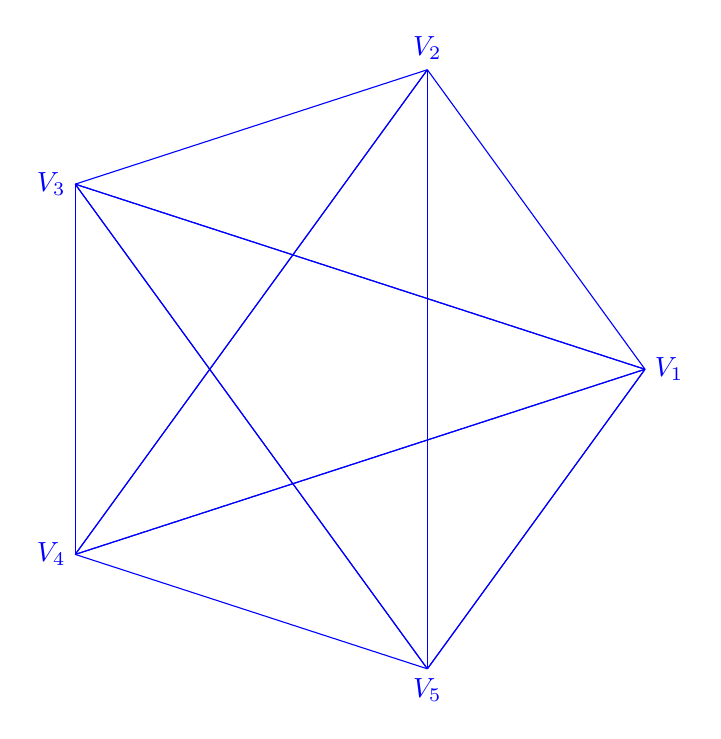
\begin{tikzpicture}[scale = 0.5]
	\pgfmathsetmacro {\n}{5};
	\pgfmathsetmacro{\p}{360/\n};
	\pgfmathsetmacro{\e}{360-\p};
    \foreach \x in {0,\p,...,\e} {
		\pgfmathsetmacro{\a}{int(round((\x + \p)/\p))};
		\newcounter{mycounter\a}
		\setcounter{mycounter\a}{\x + \p}
		\ifnum \value{mycounter\a} < 181 {
			\ifnum \value{mycounter\a} < 45
			\draw[blue] (\x:8cm)  -- (\x+ \p:8cm) node [at start,right] {$V_{\a}$};
			\else
				\ifnum \value{mycounter\a} < 135
				\draw[blue] (\x:8cm)  -- (\x+ \p:8cm) node [at start,above] {$V_{\a}$};
				\else
				\draw[blue] (\x:8cm)  -- (\x+ \p:8cm) node [at start,left] {$V_{\a}$};
				\fi
			\fi
		}
		\else {
			\ifnum \value{mycounter\a} < 225
			\draw[blue] (\x:8cm)  -- (\x+ \p:8cm) node [at start,left] {$V_{\a}$};
			\else
				\ifnum \value{mycounter\a} < 315
				\draw[blue] (\x:8cm)  -- (\x+ \p:8cm) node [at start,below] {$V_{\a}$};
				\else
				\draw[blue] (\x:8cm)  -- (\x+ \p:8cm) node [at start,right] {$V_{\a}$};
				\fi
			\fi
		}
		\fi
		\pgfmathsetmacro{\d}{\x + 2*\p};
		\pgfmathsetmacro{\n}{\x + 3*\p};
		\foreach \y in {\d,\n,...,\e} {
   			\draw[blue] (\x:8cm) -- (\y:8cm);
		}
	}
\end{tikzpicture}
\end{document}
